% !TeX root = ../../tesis.tex

% -----------------------------------------------------------------------
\subsection{Eficiencia Urbana}
\label{subsec:eficiencia-urbana}
% -----------------------------------------------------------------------

\subsubsection{Eficiencia Topológica y Caminos Mínimos}
\label{subsubsec:eficiencia-topologica}

La eficiencia de una red de transporte se entiende, en su dimensión topológica,
como la capacidad del sistema para conectar cualquier par de puntos
origen-destino a través del camino de menor costo posible ---medido en términos
de tiempo de viaje, número de transbordos o distancia recorrida---. Esta
propiedad es directamente computable sobre el grafo de la red mediante
algoritmos de caminos mínimos, lo que la convierte en una de las métricas más
operativas del análisis propuesto en este trabajo.

\citet{fortin2016innovative} plantean que los indicadores derivados de la teoría
de grafos ---como el \termino{índice alfa} (grado de ciclicidad), el
\termino{índice gamma} (grado de conectividad) y el
\termino{índice de superposición de líneas}--- caracterizan la eficiencia del
diseño de la red de manera directamente relacionada con su topología. Sin
embargo, estos autores reconocen que tales indicadores no consideran las
características únicas del transporte público, como la frecuencia de servicio,
la posibilidad de transferencias entre líneas o la variabilidad del servicio a
lo largo del día; por ello proponen complementarlos con indicadores dinámicos
derivados del modelo de grafo expandido en el tiempo construido con datos
\gtfs{}. En este modelo, la eficiencia se mide a través del camino mínimo
ponderado en la dimensión temporal, que incorpora tiempos de espera y
frecuencias reales de cada línea.

\citet{mishra2015} introducen el concepto de \termino{índice de conectividad}
nodal como medida de desempeño que trasciende la centralidad tradicional. El
índice se define como la suma de las potencias de conexión de todas las líneas
que pasan por un nodo; la potencia de cada línea pondera sus características
operativas ---velocidad, capacidad, frecuencia, tiempo de encabezamiento (
\textit{headway}) y distancia desde el origen---. Eficiencia topológica y
eficiencia operativa quedan así integradas en una métrica nodal computable que
el presente trabajo adopta como referencia para la construcción de indicadores.

\subsubsection{Centralidad de Intermediación y Congestión de Rutas}
\label{subsubsec:centralidad-intermediacion}

La distribución de los flujos de tráfico a lo largo de la red determina, en gran
medida, su eficiencia operativa. Un sistema topológicamente bien diseñado puede
resultar ineficiente en la práctica si los flujos de demanda se concentran
desproporcionadamente sobre un subconjunto reducido de nodos o aristas,
generando congestión y tiempos de viaje superiores a los predichos por el modelo
teórico.

\citet{batista2015} proponen abordar este problema mediante una variación
ponderada de la \termino{centralidad de intermediación} (
\textit{betweenness centrality}), en la que el grafo de la red vial es ponderado
no solo por la longitud de las aristas, sino por el número de rutas generadas
por la demanda real de tráfico, representada mediante una matriz origen-destino
(\textsc{od}). En su marco teórico, un nodo o arista de alta centralidad de
intermediación es aquel que aparece con mayor frecuencia en los caminos mínimos
entre los pares origen-destino del sistema; los nodos con esta propiedad
concentran los flujos de manera natural y son, por tanto, los primeros en
colapsar ante un incremento de demanda o una perturbación. La eficiencia urbana
aumenta cuando el sistema logra redistribuir estos flujos hacia rutas
alternativas, reduciendo la dependencia de los nodos centrales y homogeneizando
la carga sobre la red.

Esta perspectiva es fundamental para el análisis de la red metropolitana objeto
del presente estudio: la identificación computacional de los arcos y nodos con
mayor centralidad de intermediación ponderada por la demanda permite señalar
aquellos segmentos del sistema donde las inversiones en infraestructura o las
modificaciones de rutas producirían las mayores ganancias en eficiencia global.

\subsubsection{Accesibilidad Espacial como Dimensión de la Eficiencia}
\label{subsubsec:accesibilidad-espacial}

La eficiencia urbana no se agota en la optimización interna de los flujos de la
red; incluye también la dimensión espacial de la \termino{accesibilidad}, es
decir, la capacidad del sistema de transporte para garantizar que cualquier
usuario, independientemente de su ubicación en el territorio, pueda alcanzar una
cantidad mínima de destinos dentro de umbrales de tiempo razonables.

\citet{fortin2016innovative} señalan que los indicadores de accesibilidad más
comunes se calculan definiendo un radio de cobertura (por ejemplo, 500 metros
como distancia caminable aceptable) alrededor de las paradas de la red, y
evaluando la proporción de población o de empleos que quedan dentro de dicha
cobertura. Sin embargo, estos autores reconocen que este enfoque estático no
incorpora la demanda real de los usuarios ---representada por sus pares
origen-destino específicos--- ni la frecuencia del servicio, lo que limita su
capacidad para reflejar la experiencia real de accesibilidad. Proponen por ello
indicadores dinámicos que, construidos sobre el grafo ponderado en el tiempo,
permiten calcular la accesibilidad real desde cualquier nodo de la red hacia
todos los demás, considerando los horarios y frecuencias del servicio. Esta
\termino{accesibilidad dinámica}, calculada algorítmicamente sobre el modelo de
grafo, constituye una medida integral de la eficiencia urbana que se incorporará
al análisis computacional de la presente investigación.

\begin{figure}[H]
   \centering
   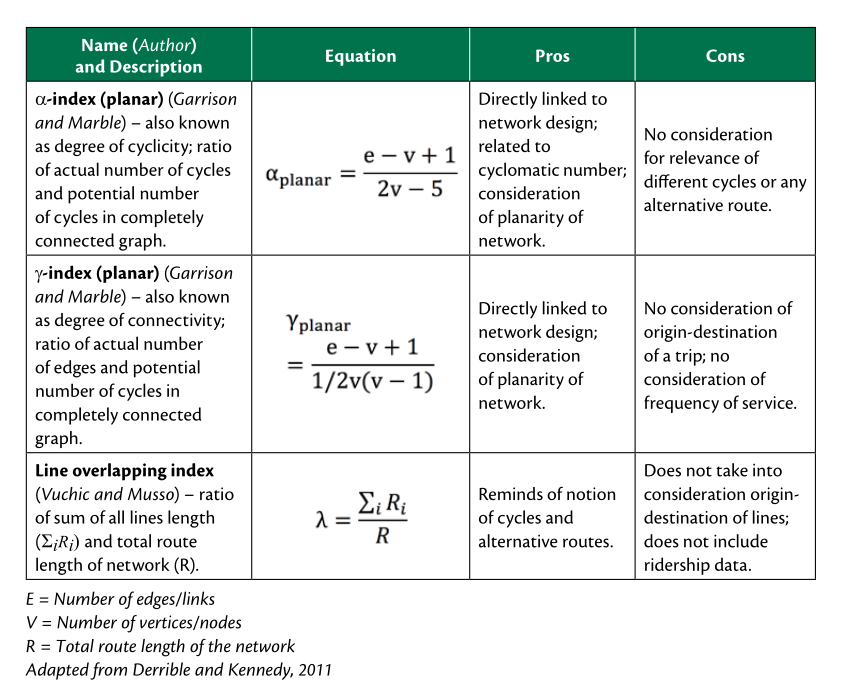
\includegraphics[width=0.85\textwidth]{Figures/Cap3/TablaIndicatorsAdaptedGraphTeory.png}
   \caption[Índices de Grafos \gtfs{}]{Tabla de indicadores de grafos \gtfs{}.}
   \label{fig:indices-grafos}
   \fuentefigura{\citet{fortin2016innovative}, p.~23.}
 \end{figure}

Los tres planos de la eficiencia aquí descritos ---topológico, operativo y
espacial--- corresponden directamente a los indicadores que el Objetivo
Específico 2 (§\ref{subsec:obj-especificos}) manda calcular: el Índice de Ruta
Directa $DI$ mide la eficiencia estructural de la topología; el Tiempo de Viaje
Promedio $T$ integra las condiciones operativas reales; y el Nivel de Cobertura
$C$ cuantifica la dimensión espacial de la accesibilidad. El cálculo conjunto de
estos tres indicadores sobre el grafo multimodal produce el diagnóstico de la
configuración actual de la red de la \zmvm{}.
